\documentclass{article}
\usepackage[utf8]{inputenc}
\usepackage[portuguese]{babel}
\usepackage[a4paper, total={7in, 9in}]{geometry}
\usepackage{graphicx}
\usepackage{float}
\usepackage[title]{appendix}
\usepackage[style=numeric]{biblatex}
\usepackage{csquotes}
\usepackage{mathtools}
\usepackage{xcolor}
\usepackage{minted}
\usepackage{framed}

\begin{document}

{
\center
\begin{figure}[H]
        \centering
        
\includegraphics[width=3cm]{Pictures/UM_EENG.jpg}
\end{figure}
\textsc{\Large Universidade do Minho} \\ [0.5cm]
\textsc{\Large Mestrado em Engenharia Informática} \\ [0.5cm]
\textsc{\large Algoritmos Paralelos} \\ [0.5cm]

{\LARGE \bfseries Problema do Caixeiro Viajante \\ usando método de Monte Carlo} \\[0.5cm]

\begin{tabular}{c c}
    José Carlos Lima Martins & Miguel Miranda Quaresma \\
    A78821 & A77049  \\
\end{tabular} \\[0.5cm]

\today \\[1cm]
}

\section{Introdução}
A resolução de diversos problemas comuns envolve, por vezes, a utilização de algoritmos/problemas de decisão que são intratáveis em tempo útil, mesmo quando 
distribuídos por diversos computadores ou unidades de processamento. Para este grupo de algoritmos, pertencentes à classe NP, não são conhecidos métodos 
determinísticos para encontrar soluções ótimas em tempo polinomial, apresentando complexidade assimptótica exponencial, sendo imperativo encontrar abordagens que permitam obter soluções em tempo útil, ainda que estas não sejam ótimas. O presente trabalho analisa duas abordagens diferentes para a resolução do problema do 
caixeiro viajante, comparando não só o desempenho das mesmas mas também a qualidade das suas soluções.

\section{Descrição do Problema}

O problema do Caixeiro Viajante (\textit{Traveling Salesman Problem - TSP}) consiste em, dado um conjunto de nodos e vértices de um grafo ligado, encontrar um caminho
que percorra todos os nodos, passando por cada um apenas uma vez, minimizando/maximizando o custo total que corresponde à soma dos vértices que formam o caminho 
escolhido. O nome que lhe é atribuído advém da analogia que se pode fazer em relação ao problema de um (Caixeiro) Viajante que pretende determinar o caminho mais curto 
entre um conjunto de cidades que pretende visitar e que passa apenas uma vez por cada cidade.

Este problema, apesar de fácil resolução para grafos com poucos nodos, aumenta exponencialmente face ao número de nodos envolvidos, apresentado complexidade
computacional fatorial: $O(N!)$. Dada a sua aplicabilidade em diversos contextos/cenários este problema é um dos problemas mais conhecidos entre os \textit{NP-Hard}.

Sendo um problema para o qual não existe um método determinístico ( limitado polinomialmente) de obter uma solução ótima, torna-se necessário desenvolver métodos
que permitam a aproximação de soluções em tempo útil. Estes métodos recorrem envolvem frequentemente o uso de algoritmos heurísticos que, apesar de não 
garantirem a obtenção de uma solução ótima, apresentam resultados que se consideram aceitáveis face ao tempo exigido para obter a solução ótima.

\subsection{Complexidade}
Como já referido anteriormente, a complexidade assimptótica do problema do Caixeiro Viajante é fatorial: $O(N!)$. Isto deve-se ao facto de que, usando um algoritmo de 
força ``bruta'' podem ser necessárias um número exponencial de operações até encontrar a solução ótima, número este que corresponde ao espaço de soluções possíveis
para o problema. Por forma a ilustrar a complexidade computacional anteriormente referida é útil descrever o algoritmo de força ``bruta'' que seria utilizado
na resolução deste problema. Este algoritmo começaria por escolher, arbitrariamente, um nodo do grafo determinando, de seguida, todas as permutações que resultariam
num caminho que percorresse todos os nodos sem repetir nenhum, permutações estas que seriam na ordem de $(n-1)!$ para um grafo com $n$ nodos. O cálculo destas 
permutações pode ser visto como o problema do caixeiro viajante aplicado a um sub-grafo contendo todos os nodos exceto o nodo inicial, aplicando-se o algoritmo de 
força ``bruta'' de maneira recursiva até não restarem mais nodos. A determinação do caminho mais curto exigiria ainda a comparação dos custos das sucessivas soluções 
(caminhos) geradas que, no pior caso, poderia exigir que todas as $n!$ soluções (caminhos) possíveis fossem geradas de maneira a encontrar o caminho mais curto, 
resultando num número de comparações proporcional ao espaço de soluções.

\section{Método de Monte Carlo}
A primeira abordagem desenvolvida para o problema envolveu o uso de uma classe de algoritmos designada métodos de Monte Carlo que permitem obter soluções aproximadas
por métodos de amostragem. Estes métodos baseam-se na tendência que a solução encontrada tem de se aproximar da solução ótima à medida que o tamanho da amostra 
aumenta. 

Um dos princípios fundamentais destes métodos consiste em realizar várias iterações sobre o problema e, em cada iteração, efetuar uma alteração local caso esta
resulte numa solução preferível ("mais ótima") à atual.
Adicionalmente, e como consequência de serem métodos probabilísticos, estes algoritmos recorrem a aleatoriedade para, em cada iteração, determinarem a ação que será
levada a cabo que, no caso do TSP, corresponde à escolha de um nodo pertencente ao caminho atual, em cada iteração.

O número de iterações/amostras efetuadas/recolhidas está ainda dependente das soluções que vão sendo geradas, sendo comum definir um número de iterações ao fim do qual
não são efetuadas mais alterações caso não se verifiquem melhorias nas soluções encontradas.

No caso do problema do Caixeiro Viajante é escolhido aleatoriamente, em cada iteração, um nodo que designaremos por \texttt{b} e, com base na sua vizinhança \textbf{i.e.} nodo anterior (\texttt{a}) e dois nodos seguintes (\texttt{c} e \texttt{d}):
\begin{enumerate}
    \item \texttt{a}
    \item \texttt{b}
    \item \texttt{c}
    \item \texttt{d}
\end{enumerate}

é determinado o impacto de alterar a ordem dos nodos de maneira a que esta seja representada por:

\begin{enumerate}
    \item \texttt{a}
    \item \texttt{c}
    \item \texttt{b}
    \item \texttt{d}
\end{enumerate}

Esta alteração consiste em trocar o nodo escolhido inicialmente (\texttt{b}) com o nodo que o precede (\texttt{c}):

\begin{figure}[H]
    \centering
    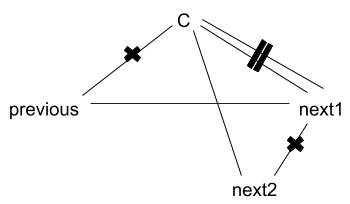
\includegraphics[width=7cm]{Pictures/montecarlo_travellingsalesman.png}
\end{figure}

Para determinar se a alteração efetuada possui um custo menor basta comparar os custos dos vértices \textbf{a-b}+\textbf{c-d} com \textbf{a-c}+\textbf{b-d} e, caso
o último apresente um valor inferior, efetuar a alteração.

\subsection{Implementação}
O algoritmo acima descrito foi desenvolvido com recurso à linguagem de programação \texttt{Haskell}, sendo implementado pela função:
\begin{verbatim}
traveling_monte_carlo :: [[Float]] -> Int -> IO (Float,[Int])
\end{verbatim}
que recebe a matriz de adjacência que representa o grafo e devolve um caminho e o respetivo custo.
Esta função começa por gerar um caminho aleatório constituído pelos nodos do grafo, invocando a função:
\begin{verbatim}
genInitialPath :: [Int] -> Int -> IO [Int]
\end{verbatim}
A função:
\begin{verbatim}
iterations :: [[Float]] -> Int -> [Int] -> Float -> Int -> Int -> IO (Float,[Int])
\end{verbatim}
é invocada de seguida que, a cada iteração, escolhe um nodo aleatório, determina os nodos adjacentes ao mesmo no caminho atual e, recorrendo à função
\begin{verbatim}
calcDelta :: (Int,Int,Int,Int) -> [Int] -> [[Float]] -> Float
\end{verbatim}
determina a variação no custo total do caminho quando é efetuada a alteração anteriormente referida.

A determinação dos nodos adjacentes é feita através da função:
\begin{verbatim}
getNeighbours :: Int -> Int -> (Int,Int,Int)
\end{verbatim}
enquanto que, a função:
\begin{verbatim}
swapNodes :: Int -> Int -> [Int] -> [Int]
\end{verbatim}
realiza a troca de dois pontos do caminho, quando essa troca proporciona uma melhoria no custo total do caminho.

Por forma a calcular o custo total do caminho, é usada a função:
\begin{verbatim}
pathCost :: Num a => [Int] -> [[a]] -> a -> a
\end{verbatim}
que é invocada para calcular o custo do caminho inicial. Este custo é atualizado quando o caminho é alterado, mediante um dado valor \texttt{delta} 
de acordo com a seguinte expressão \texttt{dist+delta}. 

\section{Simulated Annealing}

\textit{Simulated Annealing} baseia-se no método anteriormente apresentado utilizando contudo algumas técnicas de forma a conseguir obter uma melhor aproximação da solução ótima.

Esta meta-heurística permite que por vezes sejam aceites alterações que, em vez de resultarem numa redução do custo total, resultam num aumento do mesmo. Esta característica possibilita que a procura pelo solução ótima seja pelo ótimo global e não local, evitando que se fique ``preso'' num ótimo local.

Esta técnica é aplicada a cada iteração do método de Monte Carlo que recebe como parâmetro adicional uma temperatura inicial que diminui a cada iteração e influencia a aceitação de soluções que apresentem soluções menos ótimas \textbf{i.e.} a sensibilidade às mesmas. Em cada iteração, e nos casos em que não ocorre uma diminuição do custo total é verificada a seguinte condição:

\begin{equation}\label{eq:sa}
temperatura > val \land e^{\frac{-delta}{temperatura}} \ge random 
\end{equation}
\hspace{4cm} com:

\hspace{4.5cm} val próximo de 0

\hspace{4.5cm} delta = custo total no novo caminho - custo total no caminho atual

\hspace{4.5cm} random = valor aleatório entre 0 e 1
\newline\newline
que, caso seja verdadeiro, é tomado como caminho atual o novo caminho sendo mantido o caminho anterior caso não se verifique.

\subsection{Implementação}

O algoritmo acima descrito, tal como o método de Monte Carlo, foi desenvolvido com recurso à linguagem de programação \texttt{Haskell}, sendo implementado pela função:
\begin{verbatim}
simulatedAnnealing :: [[Float]] -> Int -> IO (Float, [Int])
\end{verbatim}
que recebe a matriz de adjacência e o número de iterações a realizar, devolvendo um caminho e o respetivo custo.

Inicialmente é gerado um caminho inicial, de forma aleatória recorrendo à função:
\begin{verbatim}
genInitialPath :: [Int] -> Int -> IO [Int]
\end{verbatim}
que recebe uma lista com os pontos e o tamanho e devolve a lista aleatória dos pontos.

Após a obtenção do caminho inicial é invocada a função:
\begin{verbatim}
optimizePath :: [[Float]] -> [Int] -> Int -> Int -> Float -> IO (Float, [Int])
\end{verbatim}
que recebe como argumentos a matriz de adjacência, o caminho inicial, o número de nodos, o número de iterações e a ``temperatura'' e devolve o caminho e o respetivo custo. 

Esta função, irá em cada iteração, escolher um ponto aleatório, gerar um threshold aleatório (random da expressão \ref{eq:sa}) e tentar otimizar usando a função \texttt{updatePath}. Caso não consiga, diminui o número de iterações, caso contrário, faz o reset do número de iterações, mantendo-se o caminho inalterado. Também em cada iteração é atualizada a temperatura. Quando o número de iterações é 0, calcula o custo através da função \texttt{pathCost} e retorna o custo e o caminho.

Como referido anteriormente, esta função realiza uma tentativa de otimizar o caminho:
\begin{verbatim}
updatePath :: [[Float]] -> [Int] -> Int -> Int -> Float -> Float -> Maybe [Int]
\end{verbatim}
em que recebe a matriz de adjacência, recebe o caminho atual, recebe o ponto escolhido, recebe a temperatura e recebe o threshold. Devolve o caminho atualizado caso consiga, caso contrário não devolve nada. 

Esta função, obtém os vizinhos do ponto escolhido através da função \texttt{getNeighbours} e calcula o delta, através da função \texttt{calcDelta}. Após o cálculo do delta verifica se o caminho melhorou ($delta < 0$) e em caso negativo verifica a expressão \ref{eq:sa}. Caso esta última também seja falsa não retorna nada, ou seja, não houve otimização. Caso um deles seja verdadeiro, realiza o swap dos pontos, através da função \texttt{swapNodes}, retornando o novo caminho.

Como já referido a seguinte função calcula os vizinhos:
\begin{verbatim}
getNeighbours :: Int -> Int -> (Int, Int, Int)
\end{verbatim}
em que recebe o ponto escolhido e o número de pontos existentes no grafo. Devolve os 3 pontos vizinhos, o que está antes do ponto escolhido, o que está depois do ponto escolhido e o que está 1 ponto a seguir ao ponto escolhido.

A seguinte função obtém o valor na matriz de adjacência:
\begin{verbatim}
edgeCost :: [[Float]] -> (Int, Int) -> Float
\end{verbatim}
em que recebe a matriz de adjacência e os indices. Devolve o valor.

Outra das funções já referidas é a que realiza a troca de pontos no caminho:
\begin{verbatim}
swapNodes :: Int -> Int -> [Int] -> [Int]
\end{verbatim}
em que recebe os dois pontos a trocar e o caminho. Devolve o caminho já com os pontos trocados.

Por fim, outra das funções referidas é a que calcula o custo do caminho:
\begin{verbatim}
pathCost :: [[Float]] -> [Int] -> Int -> Float
\end{verbatim}
em que recebe a matriz de adjancência, o caminho e o número de pontos do caminho. Devolve o custo do caminho.

\section{Comparação das Abordagens}

Por forma a correr as duas versões, de acordo com o PARtravelling fornecido pelo professor, foi criado uma função:
\begin{verbatim}
parallelTravel :: Int -> Int -> Int -> IO ()
\end{verbatim}
que recebe o número de nodos do grafo, o número de iterações máximo(tamanho da amostra) e o número de vezes que serão executados cada um dos dois métodos (Monte Carlo 
e Simulated Annealing). 

Esta função começa por gerar os nodos como pontos de um quadrado de lado 10 calculando de seguida a matriz de adjacência, constituída pela distância entre
os nodos (pontos), invocando a função \texttt{genGraph}. De seguida executa cada um dos métodos um número de vezes igual ao especificado pelo parâmetro referido. 

A função \texttt{genGraph}, que recebe como argumento o número de nodos, começa por gerar pontos (as suas coordenadas dentro de um quadrado de lado 10) através da 
função \texttt{genPoints}, que recebe o número de nodos e que devolve uma lista de pontos com coordenadas geradas aleatoriamente. De seguida é calculada a matriz de 
adjacência com recurso à função \texttt{graphNode}, que recebe uma lista de pontos, calcula a distância de todos esses pontos a outro ponto, passado como argumento, utilizando a função \texttt{nodeDist} que calcula a distância euclidiana entre dois pontos $P_1 (x_1, y_1)$ e $P_2 (x_2, y_2)$ tal que: 
$$ dist(P_1, P_2) = \sqrt{(x_1-x_2)^2+(y_1-y_2)^2}$$.

\subsection{\textit{Benchmarking} - Metodologia de Experimentação}
A comparação entre ambas abordagens foi feita realizando um conjunto de \textit{benchmarks} variando os parâmetros do problema \textbf{i.e.} número de iterações e 
número de nodos. Para cada uma das versões foram efetuadas 15 execuções de cada método, permitindo normalizar os valores obtidos ao reduzir a influência de 
\textit{outliers}, tendo sido tomada a mediana das execuções como tempo de execução de cada método.

\subsection{Qualidade das Soluções}
Uma observação inicial dos resultados, e tendo apenas em conta a qualidade das soluções obtidas (\textbf{i.e.} quão reduzido é o custo do caminho devolvido por cada
método) permite concluir de imediato que a abordagem de \textit{Simulated Annealing} apresenta resultados tendencialmente melhores nas diferentes versões. Isto 
pode ser facilmente justificado pelo facto de que, a aceitação de decisões que não são localmente ótimas, permite uma exploração mais abrangente/exaustiva do espaço 
de soluções, podendo levar a soluções que são mais ótimas globalmente. É importante salientar que, como foi referido, as soluções tendem a ser ótimas não sendo
certo que o sejam, algo que advém da natureza probabilística destes métodos.

\begin{figure}[H]
    \centering
    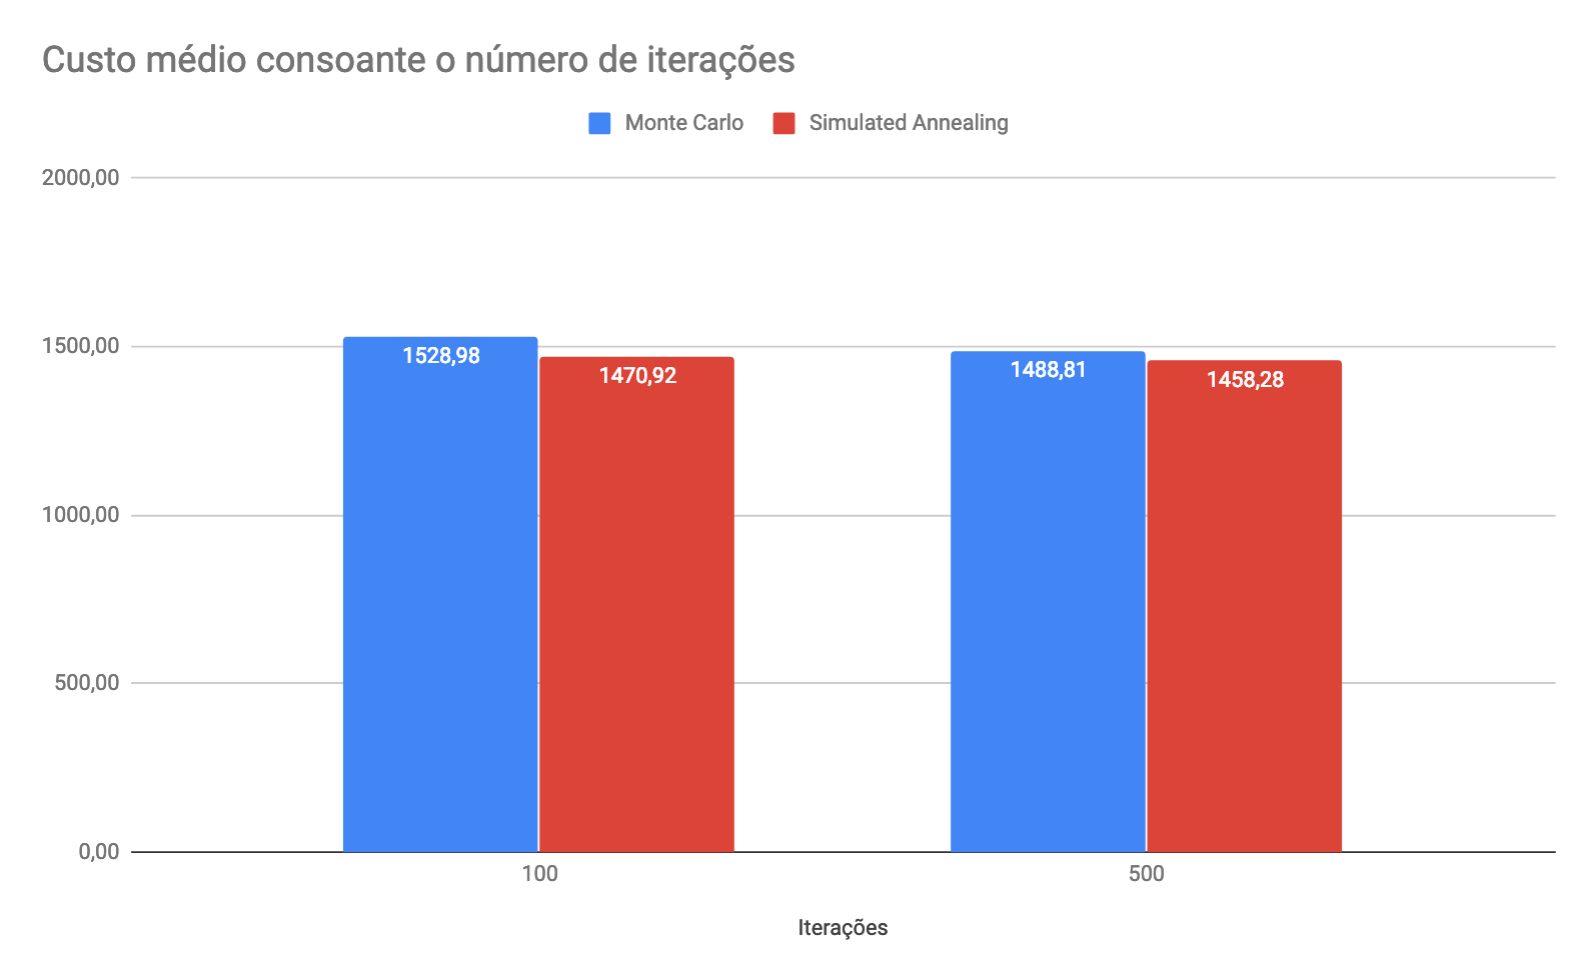
\includegraphics[width=7cm]{Pictures/AvgCost.png}
\end{figure}

O gráfico anteriormente apresentado mostra claramente a tendência para a solução ótima com o aumento do número de iterações. Adicionalmente é possível observar que, como referido, as soluções obtidas com o método de \textit{Simulated Annealing} apresentam custos inferiores ao método de Monte Carlo.

\subsection{Tempos de Execução}
Outro aspeto importante quando se comparam abordagens a problemas desta natureza consiste em analisar os tempos de execução dos diferentes métodos usados.
Neste caso é visível que o método de Monte Carlo tende a apresentar tempos de execução inferiores à abordagem com \textit{Simulated Annealing}, fenómeno
que é atribuído ao facto de, tendencialmente, serem testadas menos soluções no primeiro método do que no segundo, levando a um tempo de execução inferior.
Adicionalmente é interessante comparar o comportamento dos métodos desenvolvidos e o valor teórico de um algoritmo de força bruta para resolver o problema
do caixeiro viajante, com complexidade exponencial face ao número de nodos $O(N!)$:

\begin{figure}[H]
    \centering
    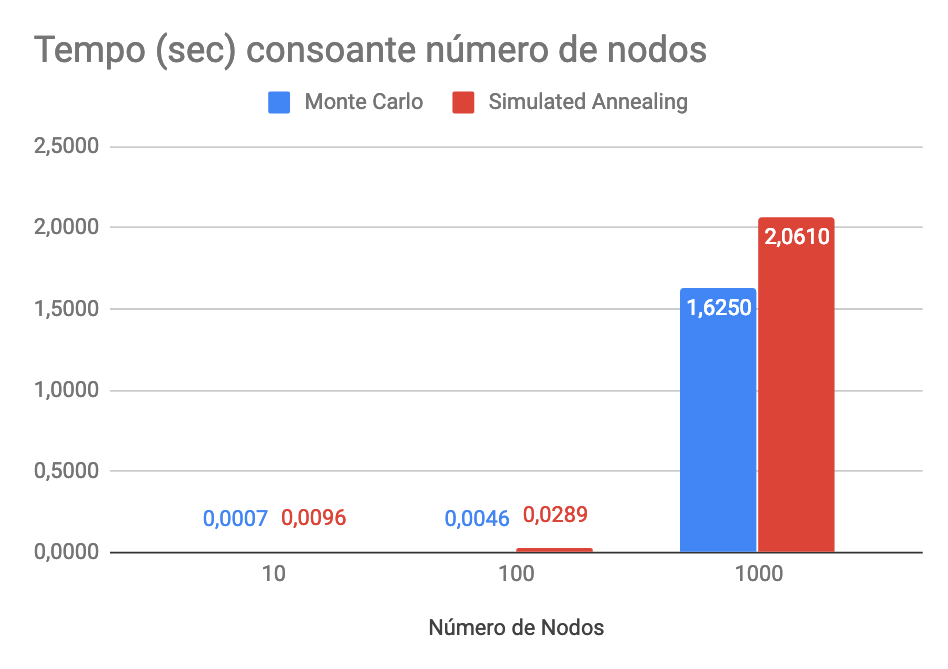
\includegraphics[width=8cm]{Pictures/ExecTimes.png}
\end{figure}

Como se pode observar, apesar do aumento no número de nodos em magnitude de ordem 10 resultar num aumento exponencial do tempo de execução, este aumento
não é de ordem fatorial, sendo por isso vantajosa a utilização de abordagens/métodos desta natureza.


\section{Conclusão}
O recursos a métodos probabilísticos é, em diversos problemas, a única abordagem que permite obter soluções aceitáveis em tempo útil. Este conjunto de métodos
é constituído por diversas abordagens que variam na qualidade das soluções obtidas sendo frequente obter soluções "mais ótimas" a troco de um tempo de execução
superior, tanto devido a um maior número de iterações como à consideração de um maior de número de soluções. Os resultados obtidos permitem concluir que a abordagem
\textit{Simulated Annealing}  apresenta soluções de maior qualidade com um aumento reduzido do tempo de execução face à abordagem com o método de Monte de Carlo.
A decisão entre ambas as abordagens não é no entanto universal, devendo ser tido em consideração o ambiente em que as mesmas irão executar (sistema embutido, supercomputador, computador pessoal, etc) e os requisitos de quem
as executa (resposta em tempo real, soluções de qualidade elevada, etc), visto que estes podem exigir tempos de execução baixos ainda que a qualidade das soluções seja inferior. Por outro lado, tratando-se de métodos 
probabilísticos, não há garantias que as soluções obtidas pelo método de \textit{Simulated Annealing} sejam sempre preferíveis às obtidas pelo método de Monte Carlo, sendo este outro fator que pode influenciar a escolha da abordagem.

\newpage 

\begin{appendices}

\section{Medianas dos Custos Obtidos}
\begin{figure}[H]
    \centering
    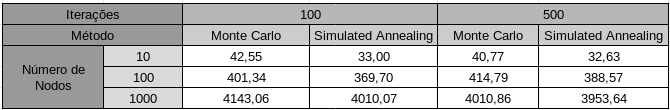
\includegraphics[width=13cm]{Pictures/custoTab.png}
\end{figure}

\section{Medianas dos Tempos de Execução Obtidos em segundos}
\begin{figure}[H]
    \centering
    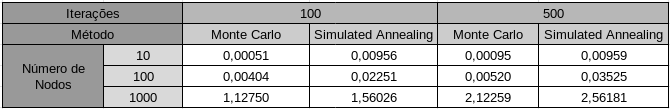
\includegraphics[width=13cm]{Pictures/tempoTab.png}
\end{figure}

\section{Código do Método de Monte Carlo}

\small
\begin{framed}
\begin{minted}{haskell}
module Monte_Carlo(traveling_monte_carlo) where
import Simulated_Annealing(genInitialPath, pathCost, getNeighbours, swapNodes, calcDelta)

import System.Random
import Data.List

traveling_monte_carlo :: [[Float]] -> Int -> IO (Float,[Int])
traveling_monte_carlo [] _ = return (0,[])
traveling_monte_carlo g it = do
                                let n = length g
                                route <- genInitialPath [0..n-1] n
                                let dist = pathCost g route n
                                retValue <- iterations g n route dist it it
                                return retValue

iterations :: [[Float]] -> Int -> [Int] -> Float -> Int -> Int -> IO (Float,[Int])
iterations _ _ route dist 0 _ = return (dist,route)
iterations graph n route dist it itStart = do
        c <- randomRIO (0,n-1)
        let (prev,n1,n2) = getNeighbours c n
        let delta = calcDelta (c,prev,n1,n2) route graph
        if delta < 0 then
            iterations graph n (swapNodes (route !! c) (route !! n1) route) (dist+delta) itStart itStart
        else
            iterations graph n route dist (it-1) itStart
\end{minted}
\end{framed}

\section{Código do Simulated Annealing}

\begin{framed}
\begin{minted}{haskell}
module Simulated_Annealing(simulatedAnnealing, pathCost, genInitialPath, getNeighbours, 
                                                           swapNodes, calcDelta) where
import System.Random
import Data.List

pathCost :: [[Float]] -> [Int] -> Int -> Float
pathCost g path nc = foldr (+) 0.0 edge_costs
            where
                edges = zip path ((tail path) ++ [head path])
                edge_costs = map (\tf -> edgeCost g tf) edges

calcDelta :: (Int,Int,Int,Int) -> [Int] -> [[Float]] -> Float
calcDelta (c,prev,n1,n2) route ll = delta
                                where
                                    pC = route !! c
                                    pPrev = route !! prev
                                    pN1 = route !! n1
                                    pN2 = route !! n2
                                    ll0 = (ll !! pPrev) !! pN1
                                    ll1 = (ll !! pC) !! pN2
                                    ll2 = (ll !! pPrev) !! pC
                                    ll3 = (ll !! pN1) !! pN2
                                    delta = (ll0 + ll1) - (ll2 + ll3)

swapNodes :: Int -> Int -> [Int] -> [Int]
swapNodes s1 s2 l = map (\x -> if x==s1 then s2 else if x==s2 then s1 else x) l

edgeCost :: [[Float]] -> (Int, Int) -> Float
edgeCost g (from, to) = (g !! from) !! to

getNeighbours :: Int -> Int -> (Int, Int, Int)
getNeighbours current n | current == n-1 = (n-2, 0, 1)
                        | current == n-2 = (n-3, n-1, 0)
                        | current == 0 = (n-1, 1, 2)
                        | otherwise =  (current-1, current+1, current+2)


updatePath :: [[Float]] -> [Int] -> Int -> Int -> Float -> Float -> Maybe [Int]
updatePath g path current nodeCount temp threshold  
    | delta < 0 || (temp > 0.001 && (exp ((-delta)/temp)) >= threshold) = updated_path
    | otherwise = Nothing
        where
            (prev, next, next_next) = getNeighbours current nodeCount
            delta = calcDelta (current, prev, next, next_next) path g
            updated_path = Just (swapNodes (path !! current) (path !! next) path)

optimizePath :: [[Float]] -> [Int] -> Int -> Int -> Int -> Float -> IO (Float, [Int])
optimizePath g path nc _ 0 _ = return (pathCost g path nc, path)
optimizePath g path nc tot_it it_left temp = do
            current <- randomRIO (0, nc-1)
            threshold <- randomRIO (0, 1.0)
            let result = updatePath g path current nc temp threshold; temp_new = temp * 0.999
            case result of
                Just path_new -> optimizePath g path_new nc tot_it tot_it temp_new
                Nothing -> optimizePath g path nc tot_it (it_left-1) temp_new

genInitialPath :: [Int] -> Int -> IO [Int]
genInitialPath [] _ = return []
genInitialPath nodes nc = do
                    n_head <- randomRIO(0, nc-1)
                    let nodes_n = swapNodes (nodes !! 0) (nodes !! n_head) nodes
                    nodes_r <- genInitialPath (tail nodes_n) (nc-1)
                    return ((nodes_n !! 0) : nodes_r)

simulatedAnnealing :: [[Float]] -> Int -> IO (Float, [Int])
simulatedAnnealing g it = do
                        let nc = length(g); nodes = [0..nc-1]
                        p <- genInitialPath nodes nc
                        optimizePath g p nc it it 1
\end{minted}
\end{framed}

\section{Código da PARtravelling}

\begin{framed}
\begin{minted}{haskell}
import Monte_Carlo(traveling_monte_carlo)
import Simulated_Annealing(simulatedAnnealing)
import System.Random
import Data.Time.Clock (diffUTCTime, getCurrentTime)

type Point = (Float, Float)

genGraph :: Int -> IO ([[Float]])
genGraph n = do
                nodes <- genPoints n
                let graph = map (graphNode nodes) [0..n-1]
                return graph

genPoints :: Int -> IO ([Point])
genPoints 0 = return []
genPoints n = do
               x <- randomRIO(0.0, 10.0)
               y <- randomRIO(0.0, 10.0)
               rest <- genPoints (n-1)
               return ((x,y) : rest)

nodeDist :: Point -> Point -> Float
nodeDist (x1,y1) (x2,y2) = sqrt ((x1-x2)^2 + (y1-y2)^2)

graphNode :: [Point] -> Int -> [Float]
graphNode nodes node = map (nodeDist (nodes !! node)) nodes

printResult :: (Float, [Int]) -> IO ()
printResult (d,p) = do
                        putStrLn ("Path found: " ++ show p)
                        putStrLn ("Total cost: " ++ show d)
                        putStrLn ""

timeFunc :: ([[Float]] -> Int -> IO (Float,[Int])) -> [[Float]] -> Int -> [Char] -> IO ()
timeFunc f graph it s = do
            start <- getCurrentTime
            result <- f graph it
            end <- getCurrentTime
            --printResult result
            putStrLn $ "Cost: " ++ show (fst result)
            putStrLn $ "Time: " ++ show (end `diffUTCTime` start)

parallelTravel :: Int -> Int -> Int -> IO ()
parallelTravel nodes it runs = do
        putStrLn (show nodes ++ " nodes, " ++ show it ++ " it, " ++ show runs ++ " runs: ")
        graph <- genGraph nodes
        putStrLn "MC:"
        mc <- sequence (replicate runs (timeFunc traveling_monte_carlo graph it "MC: "))
        putStrLn ""
        putStrLn "SA:"
        sa <- sequence (replicate runs (timeFunc simulatedAnnealing graph it "SA: "))
        putStrLn ""

main = do
    parallelTravel 10 100 15
    parallelTravel 100 100 15
    parallelTravel 1000 100 15
    parallelTravel 10 500 15
    parallelTravel 100 500 15
    parallelTravel 1000 500 15
\end{minted}
\end{framed}

\end{appendices}

\end{document}
